





























\appendix



\section{Frequently Asked Questions}

\subsection{Does DIFUSCO rely on high-quality solutions collected in advance?}

DIFUSCO does not require exact optimal solutions to train the diffusion model-based solver. For instance, in TSP-500/1000/10000, we utilize the heuristic solver LKH-3 to generate near-optimal solutions, which is nearly as fast as the neural solvers themselves (refer to Table 2 for details). Empirically (in TSP-500/1000/10000), DIFUSCO still attains state-of-the-art performance even when trained on such near-optimal solutions rather than on exact optimal ones. The training data sizes are reported in Appendix~\ref{app:evaluation}.


\subsection{This work simply applies discrete diffusion models to combinatorial optimization problems. Could you clarify the significance of this work in the field?}

It is essential to highlight that our work introduces a novel approach to solving NP-complete problems using graph-based diffusion models. This approach has not been previously explored in the context of NP-complete problems, and we believe that the significant improvements in performance over the state-of-the-art on benchmark datasets emphasize the value of our work.

Drawing a parallel to the application of diffusion models in image generation and subsequent extension to videos, our work explores a similar expansion of the scope. While denoising diffusion models have been extensively researched and applied to image generation, DIFUSCO represents the first instance where these models are applied to NP-complete CO problems. Such novelty in problem formulation is fundamental for solving NP-complete problems instead of incremental ones from a methodological point of view.

The formulation of NP-complete problems into a discrete $\{0, 1\}$-vector space and the use of graph-based denoising diffusion models to generate high-quality solutions make our approach unique. Additionally, we explore diffusion models with Gaussian and Bernoulli noise and introduce an effective inference schedule to improve the generation quality, which further underlines the significance of our work.

In conclusion, we believe that our work makes a significant and novel contribution to the field by introducing a new graph-based diffusion framework for solving NP-complete problems. The application of diffusion models, which have been primarily used for image and video generation, to the realm of combinatorial optimization highlights the innovative aspects of our research. We hope that this clarification demonstrates its importance in the field.

\subsection{How can DIFUSCO produce diverse multimodal output distribution?}

Such ability comes from the characteristics of diffusion models, which are known for generating a wide variety of distributions as generative models (like diverse images). A more comprehensive understanding can be found in the related literature, such as DDPM.

\subsection{Why is there no demonstration for the time-cost in the results shown in Table 1, and why are there some conflicts in the metrics of Length and Gaps?}

The time is not reported in Table 1 as these baseline methods are evaluated on very different hardware, which makes the runtime comparison not too meaningful. As for the “conflicts”, the results (both length and optimality gap) of all the baseline methods are directly copied from previous papers. The “conflicts” may be caused by rounding issues when reporting numerical numbers in previous papers, as our best guess.

The -0.01 gap in DIFUSCO is because the Concorde solver only accepts integer coordinates as the inputs, which may lead it to produce inaccurate non-optimal solutions due to rounding issues.

\subsection{How can we effectively evaluate the usefulness of the proposed method when the training time is also a consideration?}

It is important to clarify that in the context of neural combinatorial optimization solvers and general machine learning research, the primary focus is typically on inference time. This is because, after the model has been trained, it can be applied to a virtually unlimited number of unseen examples (graphs) during deployment. On the other hand, the training time is often considered negligible in comparative evaluations, partly due to the fact that traditional NCP solvers are hand-crafted instead of learning-based, and partly because the training cost for learnable models is out weighted by the benefits of their numerous applications.

\subsubsection{Can you name a real application that has many test instances and require such a model?}

It is worth noting that the routing problem is a fundamental and perhaps the most important combinatorial optimization problem in real-world scenarios. One example is the food delivery problem, where a pizza shop is planning to deliver pizzas to four different addresses and then return to the store. The routing problem has significant implications for industries such as retail, quick service restaurants (QSRs), consumer packaged goods (CPG), and manufacturing. In 2020, parcel shipping exceeded 131 billion in volume globally and is projected to more than double by 2026 \citep{pitneyindex}. With the changing economic and geopolitical landscape within the transport and logistics industry, Last Mile Delivery (LMD) has become the most expensive portion of the logistics fulfillment chain, representing over 41\% of overall supply chain costs \citep{lastmile}.

\begin{figure*}[t]
    \centering
    \begin{subfigure}[t]{0.48\textwidth}
    \centering
    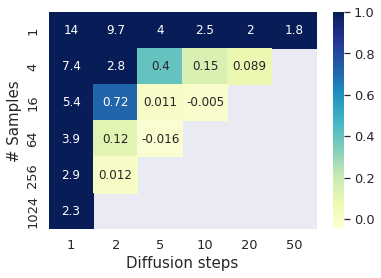
\includegraphics[width=0.8\linewidth]{gaussian_gap_orig.png}
    \vspace{-5px}
    \caption{}\label{fig:gaussian_gap_orig}
    \end{subfigure}\hfill
    \begin{subfigure}[t]{0.48\textwidth}
    \centering
    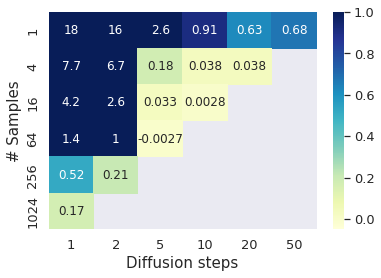
\includegraphics[width=0.8\linewidth]{bernoulli_gap_orig.png}
    \vspace{-5px}
    \caption{}\label{fig:bernoulli_gap_orig}
    \end{subfigure}
    \vspace{-5px}
    \caption{The performance $\mathrm{Gap}$ (\%) of continuous diffusion \textbf{(a)} and discrete diffusion \textbf{(b)} models on TSP-50 with different diffusion steps and number of samples. \textbf{(c)}: The results are reported with greedy decoding without 2-opt post-processing.}
    \label{fig:gap_orig}
\end{figure*}

\begin{figure*}[t]
    \centering
    \begin{subfigure}[t]{0.33\textwidth}
    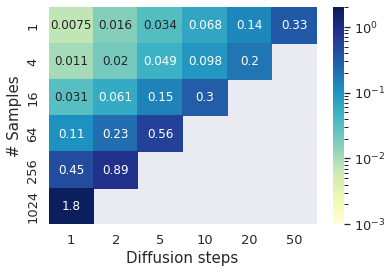
\includegraphics[width=\linewidth]{nn_latency.png}
    \vspace{-0.1in}
    \caption{}\label{fig:nn_latency}
    \end{subfigure}\hfill
    \begin{subfigure}[t]{0.33\textwidth}
    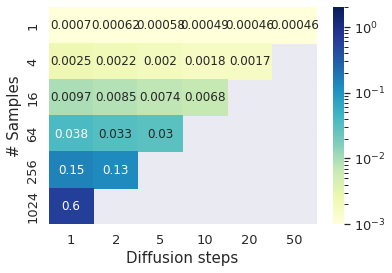
\includegraphics[width=\linewidth]{greedy_decoding_latency.png}
    \vspace{-0.1in}
    \caption{}\label{fig:greedy_decoding_latency}
    \end{subfigure}\hfill
    \begin{subfigure}[t]{0.33\textwidth}
    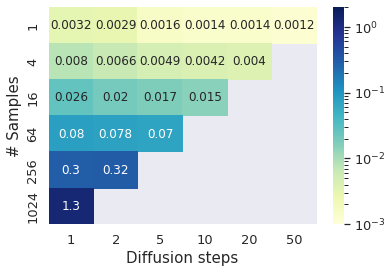
\includegraphics[width=\linewidth]{2opt_latency.png}
    \vspace{-0.1in}
    \caption{}\label{fig:2opt_latency}
    \end{subfigure}
    \vspace{-0.1in}
    \caption{The inference per-instance run-time ($\mathrm{sec}$) of diffusion models on TSP-50, where the total run-time is decomposed to neural network \textbf{(a)} + greedy decoding \textbf{(b)} + 2-opt \textbf{(c)}.}
    \label{fig:runtime_analysis}
\end{figure*}

\begin{figure}[t]
    \begin{subfigure}[t]{0.5\textwidth}
    \centering
    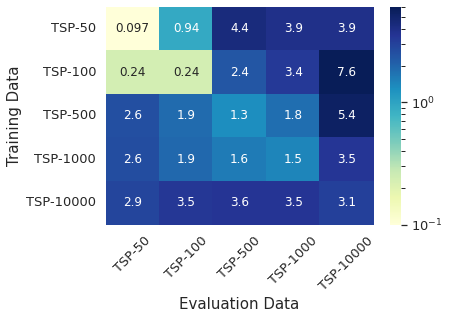
\includegraphics[width=0.8\linewidth]{generalization_2opt.png}
    \caption{}\label{fig:generalization_2opt_full}
    \end{subfigure}
    \hfill
    \begin{subfigure}[t]{0.5\textwidth}
    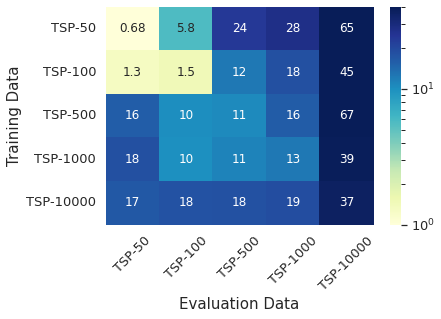
\includegraphics[width=0.8\linewidth]{generalization_orig.png}
    \centering
    \caption{}\label{fig:generalization_orig_full}
    \end{subfigure}
    \vspace{-0.1in}
    \caption{Generalization tests of discrete \method{} trained and evaluated on TSP problems across various scales. The results are reported with \textbf{(a)} and without \textbf{(b)} 2-opt post-processing.}
    \label{fig:generalization_test_full}
\end{figure}

\begin{table}[t]
\centering
\caption{Comparing discrete diffusion and continuous diffusion on TSP-100 with various diffusion steps and numbers of parallel sampling. \texttt{cosine} schedule is used for fast sampling.}
\label{tab:tsp100_compare}
\resizebox{\linewidth}{!}{
\begin{sc}
\begin{tabular}{ccccccccc}
\toprule
\small
\multirow{2}*{Diffusion Steps} & \multirow{2}*{\#Sample}
&\multicolumn{2}{c}{Discrete Diffusion ($\mathrm{Gap\%}$)}&\multicolumn{2}{c}{Continuous Diffusion ($\mathrm{Gap\%}$)} & \multicolumn{3}{c}{Per-instance runtime ($\mathrm{sec}$)}\\
& & w/ 2opt & w/o 2opt & w/ 2opt & w/o 2opt & NN & GD & 2-OPT \\
\midrule
50 & 1
& 0.23869  & 1.45574  & 1.46146 & 7.66379 & 0.50633 & 0.00171 & 0.00210    \\
100 & 1
& 0.23366  & 1.48161  & 1.32573 & 7.02117 & 1.00762 & 0.00170 & 0.00207    \\
50 & 4
& 0.02253  & 0.09280  & 0.42741 & 1.65264 & 1.52401 & 0.00643 & 0.00575    \\
10 & 16
& -0.01870 & 0.00519  & 0.13015 & 0.54983 & 1.12550 & 0.02581 & 0.02228    \\
50 & 16
& -0.02322 & -0.00699 & 0.09407 & 0.30712 & 5.63712 & 0.02525 & 0.02037    \\  
 \bottomrule
\end{tabular}
\end{sc}
}
\end{table}

\begin{table}[h]
\centering
\small
\caption{Comparison to DIMES w/ 2-opt}
\begin{sc}
\begin{tabular}{lccccccc}
\toprule
& & \multicolumn{2}{c}{TSP-500} & \multicolumn{2}{c}{TSP-1000} & \multicolumn{2}{c}{TSP-10000} \\ 
& & $\mathrm{Length}$ & $\mathrm{Gap}$ & $\mathrm{Length}$ & $\mathrm{Gap}$ & $\mathrm{Length}$ & $\mathrm{Gap}$ \\ 
\midrule
DIMES & RL+S+2opt & 17.63 & 6.52\% & 24.81 & 7.31\% & 77.18 & 7.54\% \\
DIMES & RL+AS+S+2opt & 17.30 & 4.53\% & 24.32 & 5.19\% & 75.94 & 5.81\% \\
DIFUSCO & SL+G+2opt & 16.80 & 1.49\% & 23.56 & 1.90\% & 73.99 & 3.10\% \\
DIFUSCO & SL+S+2opt & 16.65 & 0.57\% & 23.45 & 1.43\% & 73.89 & 2.95\% \\
\bottomrule
\end{tabular}
\end{sc}
\label{tab:dimes_2opt}
\end{table}


\section{Extended Related Work} \label{app:related_work}

\paragraph{Autoregressive Constructive Solvers}

Since \citet{bello2016neural} proposed the first autoregressive CO solver, more advanced models have been developed in the years since \citep{ean, 19iclr-am, peng2019deep, drori2020learning, kwon2021matrix}, including better network backbones \citep{vaswani2017attention,19iclr-am,bresson2018experimental}), more advanced deep reinforcement learning algorithms \citep{khalil2017learning,ma2019combinatorial,kool2019buy,kwon2020pomo,ouyang2021improving,xin2021multi,wang2021game,choo2022simulationguided}, improved training strategies \citep{kim2022symnco,bilearning}, and for a wider range of NPC
problems such as Capacitated Vehicle Routing Problem (CVRP) \citep{nazari2018reinforcement}, Job Shop Scheduling Problem (JSSP) \citep{zhang2020learning,park2021learning}, Maximal Independent Set (MIS) problem \citep{khalil2017learning,ahn2020learning,malherbe2022optimistic,qiudimes}, and boolean satisfiability problem (SAT) \citep{yolcu2019learning}.


\paragraph{Improvement Heuristics Solvers}

Unlike construction heuristics, DRL-based improvement heuristics solvers use neural networks to iteratively enhance the quality of the current solution until the computational budget is exhausted. Such DRL-based improvement heuristics methods are usually inspired by classical local search algorithms such as 2-opt \citep{croes1958method} and the large neighborhood search (LNS) \citep{shaw1997new}, and have been demonstrated with outstanding results by many previous works \citep{chen2019learning,hottung2019neural,da2020learning,d2020learning,xin2021neurolkh,ma2021learning,wu2021learning,l2i,wang2021bi,kim2021learning,hudson2022graph}.


Improvement heuristics methods, while showing superior performance compared to construction heuristics methods, come at the cost of increased computational time, often requiring thousands of actions even for small-scale problems with hundreds of nodes \citep{d2020learning,wang2021bi}. This is due to the sequential application of local operations, such as 2-opt, on existing solutions, resulting in a bottleneck for latency. On the other hand, \method{} has the advantage of denoising all variables in parallel, which leads to a reduction in the number of network evaluations required.



\paragraph{Continuous Diffusion Models}

Diffusion models were first proposed by \citet{sohl2015deep} and recently achieved impressive success on various tasks, such as high-resolution image synthesis \citep{dhariwal2021diffusion,ho2022cascaded}, image editing \citep{meng2021sdedit,saharia2022palette}, text-to-image generation \citep{nichol2021glide,saharia2022photorealistic,rombach2022high,ramesh2022hierarchical,gu2022vector}, waveform generation \citep{chen2020wavegrad,chen2021wavegrad,liu2022diffsinger}, video generation \citep{ho2022video,ho2022imagen,singer2022make}, and molecule generation \citep{xu2021geodiff,hoogeboom2022equivariant,wu2022diffusion}.

Recent works have also drawn connections to stochastic differential equations (SDEs) \citep{song2021score} and ordinary differential equations (ODEs) \citep{song2021denoising} in a continuous time framework, leading to improved sampling algorithms by solving discretized SDEs/ODEs with higher-order solvers \citep{liu2021pseudo,lu2022dpmpp,lu2022dpm} or implicit diffusion \citep{song2021denoising}.


\section{Additional Results}

\paragraph{Discrete Diffusion v.s. Continuous Diffusion on TSP-100}
We also compare discrete diffusion and continuous diffusion on the TSP-100 benchmark and report the results in Tab.~\ref{tab:tsp100_compare}. We can see that on TSP-100, discrete diffusion models still consistently outperform their continuous counterparts in various settings.

\paragraph{More Diffusion Steps v.s. More Sampling (w/o 2-opt)} 
Fig.~\ref{fig:gap_orig} report the results of continuous diffusion and discrete diffusion with various diffusion steps and numbers of parallel sampling, without using 2-opt post-processing. The \texttt{cosine} denoising schedule is used for fast inference. Again, we find that discrete diffusion outperforms continuous diffusion across various settings. 

Besides, we find that without the 2-opt post-processing, performing more diffusion iterations is much more effective than sampling more solutions, even when the former uses less computation. For example, $20\ (\text{diffusion steps}) \times 4 \ (\text{samples})$ not only significantly outperforms $1\ (\text{diffusion steps}) \times 1024\ (\text{samples})$, but also has a $18.5\times$ less runtime.

\paragraph{Runtime Analysis}
We report the decomposed runtime (neural network + greedy decoding + 2-opt) for diffusion models on TSP-50 in Fig.~\ref{fig:runtime_analysis}. We can see that while neural network execution takes the majority of total runtime, 2-opt also takes a non-negligible portion of the runtime, especially when only a few diffusion steps (like 1 or 2) are used.

\paragraph{Generalization Tests (w/o 2opt)}
We also report the generalization tests of discrete \method{} without 2-opt post-processing in Fig.\ref{fig:generalization_test_full} (b).

\paragraph{Comparison to DIMES w/ 2opt}

We compare DIMES with 2-opt to DIFUSCO in Tab.~\ref{tab:dimes_2opt}. We can see that while 2-opt can further improve the performance of DIMES on large-scale TPS problem instances, there is still a significant gap between DIEMS and DIFUSCO when both are equipped with 2-opt post-processing.


\setlength{\tabcolsep}{2pt}
\begin{table}[t]
    \small
    \centering
    \caption{Solution quality and computation time for learning-based methods using models trained on synthetic data (all the other baselines are trained with TSP-100) and evaluated on TSPLIB instances with 50 to 200 nodes and 2D Euclidean distances. Other baseline results are taken from \citet{hudson2022graph}.
    }
\centering
\resizebox{\linewidth}{!}{
\begin{tabular}{lcccccccccccc}
\toprule
Method  & \multicolumn{2}{c}{Kool et al.} & \multicolumn{2}{c}{Joshi et al.} & \multicolumn{2}{c}{O. da Costa et al.} & \multicolumn{2}{c}{Hudson et al.} & \multicolumn{2}{c}{Ours (TSP-50)} & \multicolumn{2}{c}{Ours (TSP-100)} \\
Instance & Time (s) & Gap (\%) & Time (s) & Gap (\%) & Time (s) & Gap (\%) & Time (s) & Gap (\%) & Time (s) & Gap (\%) & Time (s) & Gap (\%) \\
\midrule
eil51     & 0.125 & 1.628 & 3.026 & 8.339 & 28.051 & 0.067 & 10.074 & \textbf{0.000} & 0.482 & \textbf{0.000} & 0.519 & 0.117 \\
berlin52  & 0.129 & 4.169 & 3.068 & 33.225 & 31.874 & 0.449 & 10.103 & 0.142 & 0.527 & \textbf{0.000} & 0.526 & \textbf{0.000} \\
st70      & 0.200 & 1.737 & 4.037 & 24.785 & 23.964 & 0.040 & 10.053 & 0.764 & 0.663 & \textbf{0.000} & 0.670 & \textbf{0.000} \\
eil76     & 0.225 & 1.992 & 4.303 & 27.411 & 26.551 & 0.096 & 10.155 & 0.163 & 0.788 & \textbf{0.000} & 0.788 & 0.174 \\
pr76      & 0.226 & 0.816 & 4.378 & 27.793 & 39.485 & 1.228 & 10.049 & 0.039 & 0.765 & \textbf{0.000} & 0.785 & 0.187 \\
rat99     & 0.347 & 2.645 & 5.559 & 17.633 & 32.188 & 0.123 & 9.948 & 0.550 & 1.236 & 1.187 & 1.192 & \textbf{0.000} \\
kroA100   & 0.352 & 4.017 & 5.705 & 28.828 & 42.095 & 18.313 & 10.255 & 0.728 & 1.259 & 0.741 & 1.217 & \textbf{0.000} \\
kroB100   & 0.352 & 5.142 & 5.712 & 34.686 & 35.137 & 1.119 & 10.317 & 0.147 & 1.252 & 0.648 & 1.235 & \textbf{0.742} \\
kroC100   & 0.352 & 0.972 & 5.641 & 35.506 & 34.333 & 0.349 & 10.172 & 1.571 & 1.199 & 1.712 & 1.168 & \textbf{0.000} \\
kroD100   & 0.352 & 2.717 & 5.621 & 38.018 & 25.772 & 0.866 & 10.375 & 0.572 & 1.226 & \textbf{0.000} & 1.175 & 0.000 \\
kroE100   & 0.352 & 1.470 & 5.650 & 26.589 & 34.475 & 1.832 & 10.270 & 1.216 & 1.208 & 0.274 & 1.197 & \textbf{0.274} \\
rd100     & 0.352 & 3.407 & 5.737 & 50.432 & 28.963 & 0.003 & 10.125 & 0.459 & 1.191 & \textbf{0.000} & 1.172 & 0.000 \\
eil101    & 0.359 & 2.994 & 5.790 & 26.701 & 23.842 & 0.387 & 10.276 & 0.201 & 1.222 & 0.576 & 1.215 & \textbf{0.000} \\
lin105    & 0.380 & 1.739 & 5.938 & 34.902 & 39.517 & 1.867 & 10.330 & 0.606 & 1.321 & \textbf{0.000} & 1.280 & \textbf{0.000} \\
pr107     & 0.391 & 3.933 & 5.964 & 80.564 & 29.039 & 0.898 & 9.977 & 0.439 & 1.381 & \textbf{0.228} & 1.378 & 0.415 \\
pr124     & 0.499 & 3.677 & 7.059 & 70.146 & 29.570 & 10.322 & 10.360 & 0.755 & 1.803 & 0.925 & 1.782 & \textbf{0.494} \\
bier127   & 0.522 & 5.908 & 7.242 & 45.561 & 39.029 & 3.044 & 10.260 & 1.948 & 1.938 & \textbf{1.011} & 1.915 & 0.366 \\
ch130     & 0.550 & 3.182 & 7.351 & 39.090 & 34.436 & 0.709 & 10.032 & 3.519 & 1.989 & \textbf{1.970} & 1.967 & 0.077 \\
pr136     & 0.585 & 5.064 & 7.727 & 58.673 & 31.056 & 0.000 & 10.379 & 3.387 & 2.184 & \textbf{2.490} & 2.142 & 0.000 \\
pr144     & 0.638 & 7.641 & 8.132 & 55.837 & 28.913 & 1.526 & 10.276 & 3.581 & 2.478 & \textbf{0.519} & 2.446 & 0.261 \\
ch150     & 0.697 & 4.584 & 8.546 & 49.743 & 35.497 & 0.312 & 10.109 & 2.113 & 2.608 & \textbf{0.376} & 2.555 & 0.000 \\
kroA150   & 0.695 & 3.784 & 8.450 & 45.411 & 29.399 & 0.724 & 10.331 & 2.984 & 2.617 & 3.753 & 2.601 & \textbf{0.000} \\
kroB150   & 0.696 & 2.437 & 8.573 & 56.745 & 29.005 & 0.886 & 10.018 & 3.258 & 2.626 & \textbf{1.839} & 2.592 & 0.067 \\
pr152     & 0.708 & 7.494 & 8.632 & 33.925 & 29.003 & 0.029 & 10.267 & 3.119 & 2.716 & \textbf{1.751} & 2.712 & 0.481 \\
u159      & 0.764 & 7.551 & 9.012 & 38.338 & 28.961 & 0.054 & 10.428 & 1.020 & 2.963 & 3.758 & 2.892 & \textbf{0.000} \\
rat195    & 1.114 & 6.893 & 11.236 & 24.968 & 34.425 & 0.743 & 12.295 & 1.666 & 4.400 & 1.540 & 4.428 & \textbf{0.767} \\
d198      & 1.153 & 373.020 & 11.519 & 62.351 & 30.864 & 0.522 & 12.596 & 4.772 & 4.615 & 4.832 & 4.153 & \textbf{3.337} \\
kroA200   & 1.150 & 7.106 & 11.702 & 40.885 & 33.832 & 1.441 & 11.088 & 2.029 & 4.710 & 6.187 & 4.686 & \textbf{0.065} \\
kroB200   & 1.150 & 8.541 & 11.689 & 43.643 & 31.951 & 2.064 & 11.267 & 2.589 & 4.606 & 6.605 & 4.619 & \textbf{0.590} \\
\midrule
Mean      & 0.532 & 16.767 & 7.000 & 40.025 & 31.766 & 1.725 & 10.420 & 1.529 & 1.999 & 1.480 & 1.966 & \textbf{0.290} \\
\bottomrule
\end{tabular}
}
\label{tab:tsplib}
\end{table}
\setlength{\tabcolsep}{6pt}


\paragraph{Generalization to Real-World Instances}\label{sec:tsplib}

In many cases, there might not be enough real-world problem instances available to train a model. As a result, the model needs to be trained using synthetically generated data. Hence, it becomes crucial to assess the effectiveness of transferring knowledge from the simulated environment to the real world. 
we evaluated the DIFUSCO models trained on TSP-50 and TSP-100 on TSPLib graphs with 50-200 nodes and a comparison to other methods (trained TSP-100) \citep{19iclr-am,joshi2019efficient,d2020learning,hudson2022graph} is shown in Tab.~\ref{tab:tsplib}.

We can see that DIFUSCO achieves significant improvements over other baselines on the real-world TSPLIB data (0.29\% gap v.s. 1.48\% in the best baseline). Besides, DIFUSCO also shows strong generalization ability across problem scales, where DIFUSCO trained on TSP-50 data achieves competitive performance with the best baseline \citet{hudson2022graph} trained on TSP-100.

\paragraph{MCTS with Multiple Diffusion Samples}

One may wonder what if DIFUSCO with MCTS is allowed to have more than one sample. To evaluate the impact of using multiple samples in DIFUSCO with MCTS, we conducted experiments with 1x, 2x, and 4x greedy heatmap generation (50 diffusion steps) combined with MCTS using different random seeds, and report the results in Tab.~\ref{tab:mcts_samples}.

Our findings show that DIFUSCO's performance significantly improves when MCTS decoding is applied to diverse heatmaps. We would like to highlight that the diverse heatmap + MCTS decoding approach is unique to diffusion model-based neural solvers like DIFUSCO, as previous methods (e.g., Att-GCN and DIMES) that employ MCTS only yield a unimodal distribution. While it is true that using 2x or 4x MCTS decoding would increase the runtime of DIFUSCO, we believe there is a similar exploitation versus exploration trade-off between MCTS time and MCTS seeds, akin to the trade-off between diffusion steps and the number of samples demonstrated in Figure 2 of our paper.

\begin{table}[t]
\centering
\small
\caption{Results of DIFUSCO with multiple samples for MCTS}
\begin{sc}
\begin{tabular}{lccccccc}
\toprule
& & \multicolumn{2}{c}{TSP-500} & \multicolumn{2}{c}{TSP-1000} & \multicolumn{2}{c}{TSP-10000} \\ 
& & $\mathrm{Length}$ & $\mathrm{Gap}$ & $\mathrm{Length}$ & $\mathrm{Gap}$ & $\mathrm{Length}$ & $\mathrm{Gap}$ \\ 
\midrule
Previous SOTA & & 16.84 & 1.76\% & 23.69 & 2.46\% & 74.06 & 3.19\% \\
DIFUSCO 1xMCTS & & 16.64 & 0.46\% & 23.39 & 1.17\% & 73.62 & 2.58\% \\
DIFUSCO 2xMCTS & & 16.57 & 0.09\% & 23.32 & 0.56\% & 73.60 & 2.55\% \\
DIFUSCO 4xMCTS & & 16.56 & 0.02\% & 23.30 & 0.46\% & 73.54 & 2.48\% \\
\bottomrule
\end{tabular}
\end{sc}
\label{tab:mcts_samples}
\end{table}


\section{Discussion on the $\{0, 1\}^N$ Vector Space of CO Problems} \label{sec:mip}

The design of the $\{0, 1\}^N$ vector space can also represent non-graph-based NP-complete combinatorial optimization problems.
For example, on the more general Mixed Integer Programming (MIP) problem, we can let $\CAL X_s$ be a 0/1 indication set of all extended variables\footnote{For an integer variable $z$ that can be assigned values from a finite set with cardinality $\mathrm{card}(z)$, any target value can be represented as a sequence of $\lceil \log_2(\mathrm{card}(z)) \rceil$ bits \citep{nair2020solving,chen2022analog}.}. $\mathrm{cost}(\cdot)$ can be defined as a linear/quadratic function of $\mathbf{x}$, and $\mathrm{valid}(\cdot)$ is a function validating all linear/quadratic constraints, bound constraints, and integrality constraints.

\section{Additional Experiment Details} \label{app:evaluation}

\paragraph{Metrics: TSP}
For TSP, Length is defined as the average length of the system-predicted tour for each test-set instance. Gap is the average of the relative decrease in performance compared to a baseline method. 
Time is the total clock time required to generate solutions for all test instances, and is presented in seconds (s), minutes (m), or hours (h).

\paragraph{Metrics: MIS}
For MIS, Size (the larger, the better) is the average size of the system-predicted maximal independent set for each test-set graph, Gap and Time are defined similarly as in the TSP case.

\paragraph{Hardware}
All the methods are trained with $8\times$ NVIDIA Tesla V100 Volta GPUs and evaluated on a single NVIDIA Tesla V100 Volta GPU, with $40\times$ Intel(R) Xeon(R) Gold 6248 CPUs @ 2.50GHz.

\paragraph{Random Seeds}

Since the diffusion models can generate an arbitrary sample from its distribution even with the greedy decoding scheme, we report the averaged results across 5 different random seeds when reporting all results.

\paragraph{Training Details}

All \method{} models are trained with a cosine learning rate schedule starting from 2e-4 and ending at 0.


\begin{itemize}[leftmargin=0.15in] \item TSP-50: We use 1502000 random instances and train \method{} for 50 epochs with a batch size of 512. \item TSP-100: We use 1502000 random instances and train \method{} for 50 epochs with a batch size of 256. \item TSP-500: We use 128000 random instances and train \method{} for 50 epochs with a batch size of 64. We also apply curriculum learning and initialize the model from the TSP-100 checkpoint. \item TSP-1000: We use 64000 random instances and train \method{} for 50 epochs with a batch size of 64. We also apply curriculum learning and initialize the model from the TSP-100 checkpoint. \item TSP-10000: We use 6400 random instances and train \method{} for 50 epochs with a batch size of 8. We also apply curriculum learning and initialize the model from the TSP-500 checkpoint. \item SATLIB: We use the training split of 49500 examples from \citep{hoos2000satlib,qiudimes} and train \method{} for 50 epochs with a batch size of 128. \item ER-[700-800]: We use 163840 random instances and train \method{} for 50 epochs with a batch size of 32. \end{itemize}


\section{Decoding Strategies} \label{app:decoding}

\paragraph{Greedy Decoding} We use a simple greedy decoding scheme for diffusion models, where we sample one solution from the learned distribution $p_{\boldsymbol{\theta}}(\mathbf{x}_0)$. We compare this scheme with other autoregressive constructive solvers that also use greedy decoding.

\paragraph{Sampling} Following \citet{19iclr-am}, we also use a sampling scheme where we sample multiple solutions in parallel (i.e., each diffusion model starts with a different noise $\mathbf{x_{T}}$) and report the best one.

\paragraph{Monte Carlo Tree Search} For the TSP task, we adopt a more advanced reinforcement learning-based search approach, i.e., Monte Carlo tree search (MCTS), to find high-quality solutions. In MCTS, we sample $k$-opt transformation actions guided by the heatmap generated by the diffusion model to improve the current solutions. The MCTS repeats the simulation, selection, and back-propagation steps until no improving actions are found in the sampling pool. For more details, please refer to \citep{fu2021generalize}.




\section{Fast Inference for Continuous and Discrete Diffusion Models} \label{app:ddim}

We first describe the denoising diffusion implicit models (DDIMs) \citep{song2021denoising} algorithm for accelerating inference for continuous diffusion models.

Formally, consider the forward process  defined not  on all the latent variables $\mathbf{x}_{1:T}$, but on a subset $\{\mathbf{x}_{\tau_1}, \dots, \mathbf{x}_{\tau_M}\}$, where $\tau$ is an increasing sub-sequence of $[1, \dots, T]$ with length $M$, $\mathbf{x}_{\tau_1} = 1$ and $\mathbf{x}_{\tau_M} = T$.

For continuous diffusion, the marginal can still be defined as:
\begin{equation}
    q(\mathbf{x}_{\tau_{i}} | \mathbf{x}_{0}) \coloneqq
    \mathcal{N}(\mathbf{x}_{\tau_i}; \sqrt{\bar{\alpha}_{\tau_i}} \mathbf{x}_0, (1 - \bar{\alpha}_{\tau_i}) \mathbf{I})
\end{equation}

And it's (deterministic) posterior is defined by:
\begin{equation}
    q(\mathbf{x}_{\tau_{i-1}} | \mathbf{x}_{\tau_{i}}, \mathbf{x}_{0}) \coloneqq
     \mathcal{N}(\mathbf{x}_{\tau_{i-1}}; 
    \sqrt{\frac{\bar{\alpha}_{\tau_{i-1}}}{\bar{\alpha}_{\tau_i}}} 
    \left(\mathbf{x}_{\tau_{i}} - \sqrt{1 - \bar{\alpha}_{\tau_i}} \cdot \widetilde{\boldsymbol{\epsilon}}_{\tau_i} \right) + \sqrt{1 - \bar{\alpha}_{\tau_{i-1}}} \cdot \widetilde{\boldsymbol{\epsilon}}_{\tau_i} )
    , \mathbf{0})
\end{equation}
where $\widetilde{\boldsymbol{\epsilon}}_{\tau_i} = {(\mathbf{x}_{\tau_i} - \sqrt{\bar{\alpha}_{\tau_i}} \mathbf{x}_0) / \sqrt{1 - \bar{\alpha}_{\tau_i}}}$ is the (predicted) diffusion noise.

Next, we describe its analogy in the discrete domain, which is first proposed by \citet{austin2021structured}.

For discrete diffusion, the marginal can still be defined as:
\begin{equation}
    q(\mathbf{x}_{\tau_{i}} | \mathbf{x}_{0}) =
    \mathrm{Cat}\left(\mathbf{x}_{\tau_i} ; \mathbf{p} =  \mathbf{x}_{0} \overline{\mathbf{Q}}_{\tau_i} \right),
\end{equation}
while the posterior becomes:
\begin{equation}\label{eq:bayes-fast}
\begin{split}
& q(\mathbf{x}_{\tau_{i-1}}|\mathbf{x}_{\tau_{i}}, \mathbf{x}_0)  = \frac{q(\mathbf{x}_{\tau_{i}}|\mathbf{x}_{\tau_{i-1}}, \mathbf{x}_0)q(\mathbf{x}_{\tau_{i-1}}|\mathbf{x}_0)}{q(\mathbf{x}_{\tau_{i}} | \mathbf{x}_0)}\\
&= \mathrm{Cat} \left(
\mathbf{x}_{\tau_{i-1}} ; \mathbf{p} = \frac{
    \mathbf{x}_{\tau_{i}} \overline{\mathbf{Q}}_{{\tau_{i-1}}, {\tau_{i}}}^{\top} \odot \mathbf{x}_0 \overline{\mathbf{Q}}_{\tau_{i-1}}
}{\mathbf{x}_0 \overline{\mathbf{Q}}_{\tau_{i}} \mathbf{x}_{\tau_{i}}^\top }
\right),
\end{split}
\end{equation}
where $\overline{\mathbf{Q}}_{t', t} = \mathbf{Q}_{t' + 1} \dots \mathbf{Q}_{t}$.


\begin{figure}[tb]
    \centering
    \includegraphics[width=\linewidth]{cotinous_steps.pdf}
    \caption{Qualitative illustration of how diffusion steps affect the generation quality of \textbf{continuous} diffusion models. The results are reported without any post-processing. \textbf{Continuous} \method{} with 50 (first row), 20 (second row), 10 (third row), and 5 (last row) diffusion steps in \texttt{cosine} schedule are shown.}
    \label{fig:cotinous_steps}
\end{figure}

\begin{figure}[tb]
    \centering
    \includegraphics[width=\linewidth]{discrete_steps.pdf}
    \caption{Qualitative illustration of how diffusion steps affect the generation quality of \textbf{discrete} diffusion models. The results are reported without any post-processing. \textbf{Discrete} \method{} with 50 (first row), 20 (second row), 10 (third row), and 5 (last row) diffusion steps in \texttt{cosine} schedule are shown.}
    \label{fig:discrete_steps}
\end{figure}

\begin{figure}[tb]
    \centering
    \includegraphics[width=\linewidth]{contnous_schedule.pdf}
    \caption{Qualitative illustration of how diffusion schedules affect the generation quality of \textbf{continuous} diffusion models. The results are reported without any post-processing. \textbf{Continuous} \method{} with \texttt{linear} schedule (first row) and \texttt{cosine} schedule (second row) with 20 diffusion steps are shown.}
    \label{fig:contnous_schedule}
\end{figure}

\begin{figure}[tb]
    \centering
    \includegraphics[width=\linewidth]{discrete_schedule.pdf}
    \caption{Qualitative illustration of how diffusion schedules affect the generation quality of \textbf{discrete} diffusion models. The results are reported without any post-processing. \textbf{Discrete} \method{} with \texttt{linear} schedule (first row) and \texttt{cosine} schedule (second row) with 20 diffusion steps are shown.}
    \label{fig:discrete_schedule}
\end{figure}

\begin{figure}[tb]
    \centering
    \includegraphics[width=\linewidth]{discrete_examples.pdf}
    \caption{Qualitative illustration of discrete \method{} on TSP-50, TSP-100 and TSP-500 with 50 diffusion steps and \texttt{cosine} schedule.}
    \label{fig:qualitative2}
\end{figure}

\begin{figure}[t]
    \centering
    \includegraphics[width=0.8\linewidth]{failure.pdf}
    \caption{Success (left) and failure (right) examples on TSP-100, where the latter fails to form a single tour that visits each node exactly once. The results are reported without any post-processing.}
    \label{fig:qualitative3}
\end{figure}


\section{Experiment Baselines} \label{app:baselines}


\paragraph{TSP-50/100} We evaluate \method{} on TSP-50 and TSP-100 against 10 baselines, which belong to two categories: traditional Operations Research (OR) methods and learning-based methods. \begin{itemize}[leftmargin=0.15in] \item Traditional OR methods include Concorde \citep{applegate2006concorde}, an exact solver, and 2-opt \citep{lin1973effective}, a heuristic method. \item Learning-based methods include AM \citep{19iclr-am}, GCN \citep{joshi2019efficient}, Transformer \citep{bresson2021transformer}, POMO \citep{kwon2020pomo}, Sym-NCO\citep{kim2022symnco}, DPDP \citep{ma2021learning}, Image Diffusion \citep{graikos2022diffusion}, and MDAM \citep{xin2021multi}. These are the state-of-the-art methods in recent benchmark studies. \end{itemize}

\paragraph{TSP-500/1000/10000}


We compare \method{} on large-scale TSP problems with 9 baseline methods, which fall into two categories: traditional Operations Research (OR) methods and learning-based methods. \begin{itemize}[leftmargin=0.15in] \item Traditional OR methods include Concorde \citep{applegate2006concorde} and Gurobi \citep{gurobi2018gurobi}, which are exact solvers, and LKH-3 \citep{lkh3}, which is a strong heuristic solver. We use two settings for LKH-3: (i) \emph{default}: 10000 trials (the default configuration of LKH-3); (ii) \emph{less trials}: 500 trials for TSP-500/1000 and 250 trials for TSP-10000. We also include Farthest Insertion, a simple heuristic method, as a baseline. \item Learning-based methods include EAN \citep{ean}, AM \citep{19iclr-am}, GCN \citep{joshi2019efficient}, POMO+EAS \citep{kwon2020pomo, hottung2021efficient}, Att-GCN \citep{fu2021generalize}, and DIMES \citep{qiudimes}. These are the state-of-the-art methods in recent benchmark studies. They can be further divided into reinforcement learning (RL) and supervised learning (SL) methods. Some RL methods can also use an Active Search (AS) stage \citep{bello2016neural} to fine-tune each instance. We take the results of the baselines from \citet{fu2021generalize} and \citet{qiudimes}. Note that except for Att-GCN and DIMES, the baselines are trained on small graphs and tested on large graphs. \end{itemize}

\paragraph{MIS} For MIS, we compare \method{} with 6 other MIS solvers on the same test sets, including two traditional OR methods (i.e., Gurobi and KaMIS) and four learning-based methods.
Gurobi solves MIS as an integer linear program, while KaMIS is a heuristics solver for MIS.
The four learning-based methods can be divided into the reinforcement learning (RL) category, i.e., LwD \citep{ahn2020learning}) and DIMES \citep{qiudimes}, and the supervised learning (SL) category, i.e., Intel \citep{li2018combinatorial} and DGL \citep{other2022whats}.




